\subsection{Etapa de Prototipação}

O protótipo da interface do usuário será desenvolvida utilizando como base o modelo utilizando no \textit{Montra}, um projeto com design free, ou seja, que pode ser utilizado por qualquer pessoa.

Todo o protótipo gerado pode ser conferido com mais detalhes no figma, \url{https://www.figma.com/file/ONcoN1mFA371DaaP44y0C1/Montra---Expense-Tracker-UI-Kit-(Community)?type=design&node-id=223-1&mode=design&t=xuHI5oFSQPix7ojR-0}.

\begin{figure}[!htb]
    \centering
    \caption{Apresentação do App}
    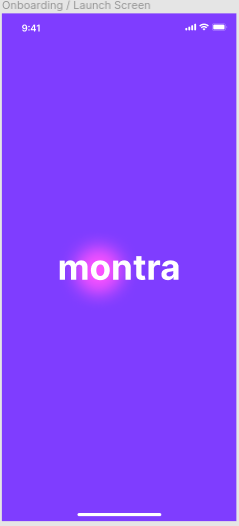
\includegraphics[scale=0.6]{images/presentation.png}
\end{figure}

\begin{figure}[!htb]
    \centering
    \caption{Página Inicial}
    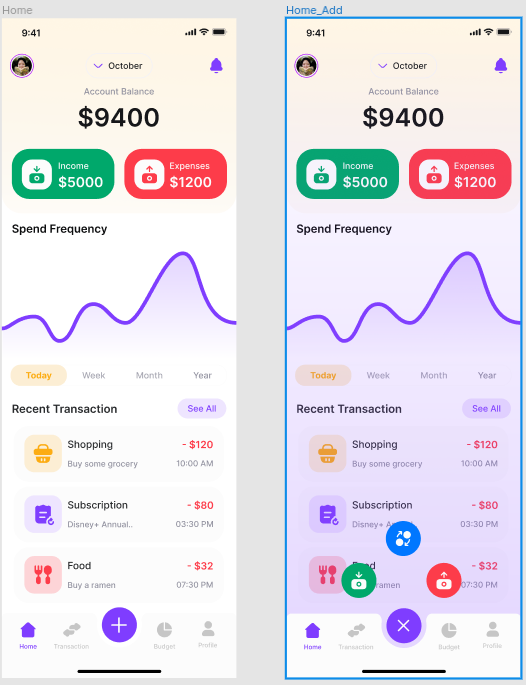
\includegraphics[scale=0.6]{images/home.png}
\end{figure}

\begin{figure}[!htb]
    \centering
    \caption{Adicionar despesa/receita}
    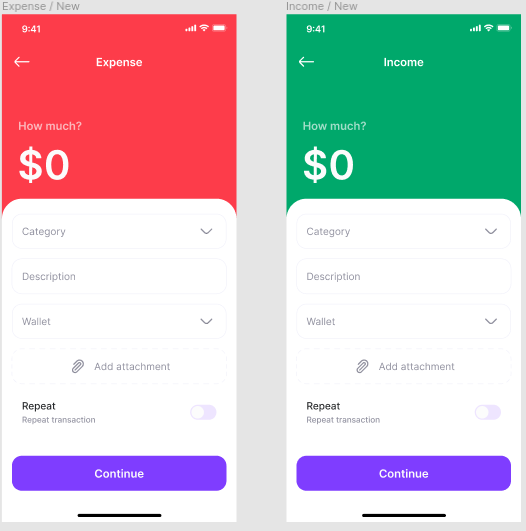
\includegraphics[scale=0.6]{images/receipts.png}
\end{figure}

\begin{figure}[!htb]
    \centering
    \caption{Notificações}
    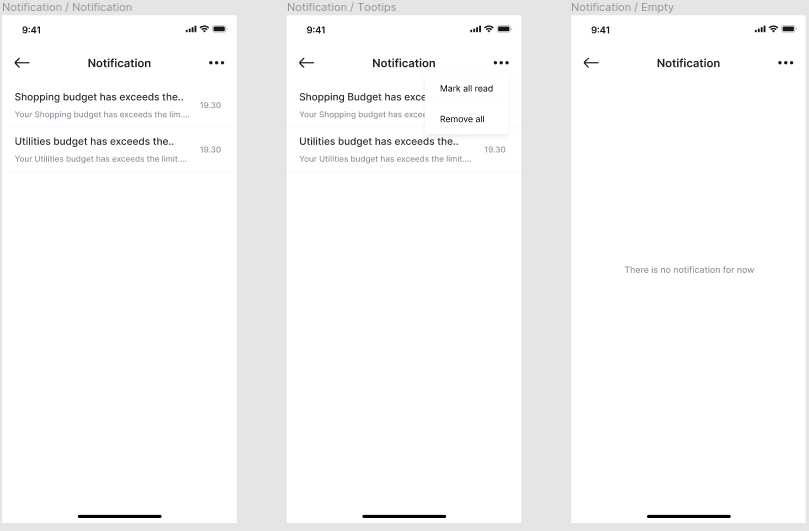
\includegraphics[scale=0.6]{images/notification.png}
\end{figure}


\begin{figure}[!htb]
    \centering
    \caption{Apresentação da tabela mensal}
    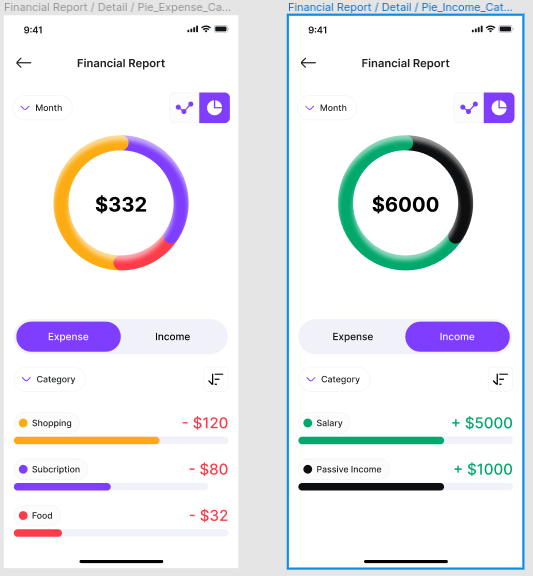
\includegraphics[scale=0.6]{images/expense-table.png}
\end{figure}

\begin{figure}[!htb]
    \centering
    \caption{Gráficos}
    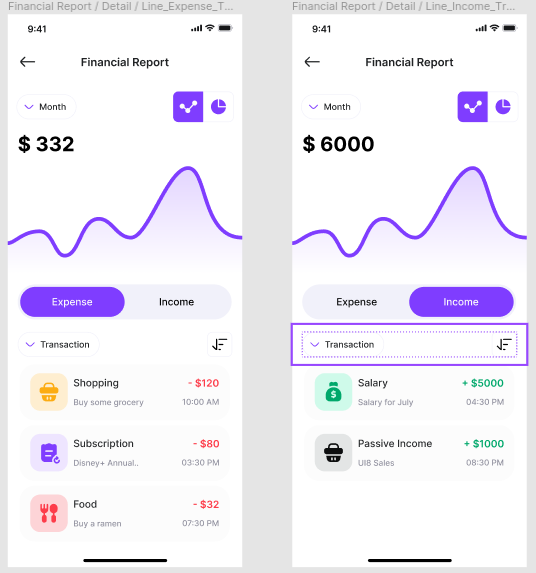
\includegraphics[scale=0.6]{images/graphic.png}
\end{figure}


As figuras mostradas foram apenas uma porção, \textit{sneakpeak} do que foi desenvolvido, o material completo pode ser encontrado no site do figma